\label{Chapter:Automated Guided Jumping}
In this chapter, we will start by discussing the interaction design for an automated guided jumping navigation technique that would meet the research questions referenced in \cref{section GJM: Conclusion}. This will be followed by details about the development of the technique, which can be divided into two parts; the setup of an environment and narrative structure for using this technique and the development of automated jumping in a way that jumps are comprehensible to users. 

\section{Interaction Design}
\label{section AGJ: Interaction Design}
Looking at the use cases and motivation discussed in \cref{Chapter:Guided Jumping Motivation} we will first lay out a scenario in which our technique would be used and then go through the interaction design of the technique based on this scenario.

\subsection{Scenario}
\label{subsection AGJ ID: Scenario}
We developed our automated guided jumping navigation technique for a virtual tour of an indoor space, which a user can do alone without a tour guide. There is potential to think of how this can be extended to a virtual tour of indoor spaces for a group of users without a tour guide as well. The goal of this virtual tour would be to explore specific objects and exhibits that could have a similar theme that a user is interested it and learn about them while also remembering what they have seen and where they saw it. 

\subsection{Exploration Steps}
\label{subsection AGJ ID: Exploration Steps}
A tour of the \acrshort{ve} would take place by ensuring that users go to specified locations of interest or nodes. Since these could be quite far from each other there should be way-points in between each node so that users would travel shorter distances to the nodes, hence, justifying the navigation being a jumping metaphor instead of teleportation. As shown in \cref{fig:interaction-design-steps}, when a user is touring the environment, they start at the first node. Here they can explore and wait for a while till they are willing to move on. When they are ready to jump, they get some form of travel feedback, so they are aware that a jump is about to take place. Then a jump takes place to either the next node or a way-point. The user can now explore and wait or again jump to the next node or way-point. On reaching the final node, the jumps would stop, and the tour would end. 

\begin{figure}[]
	\centering
	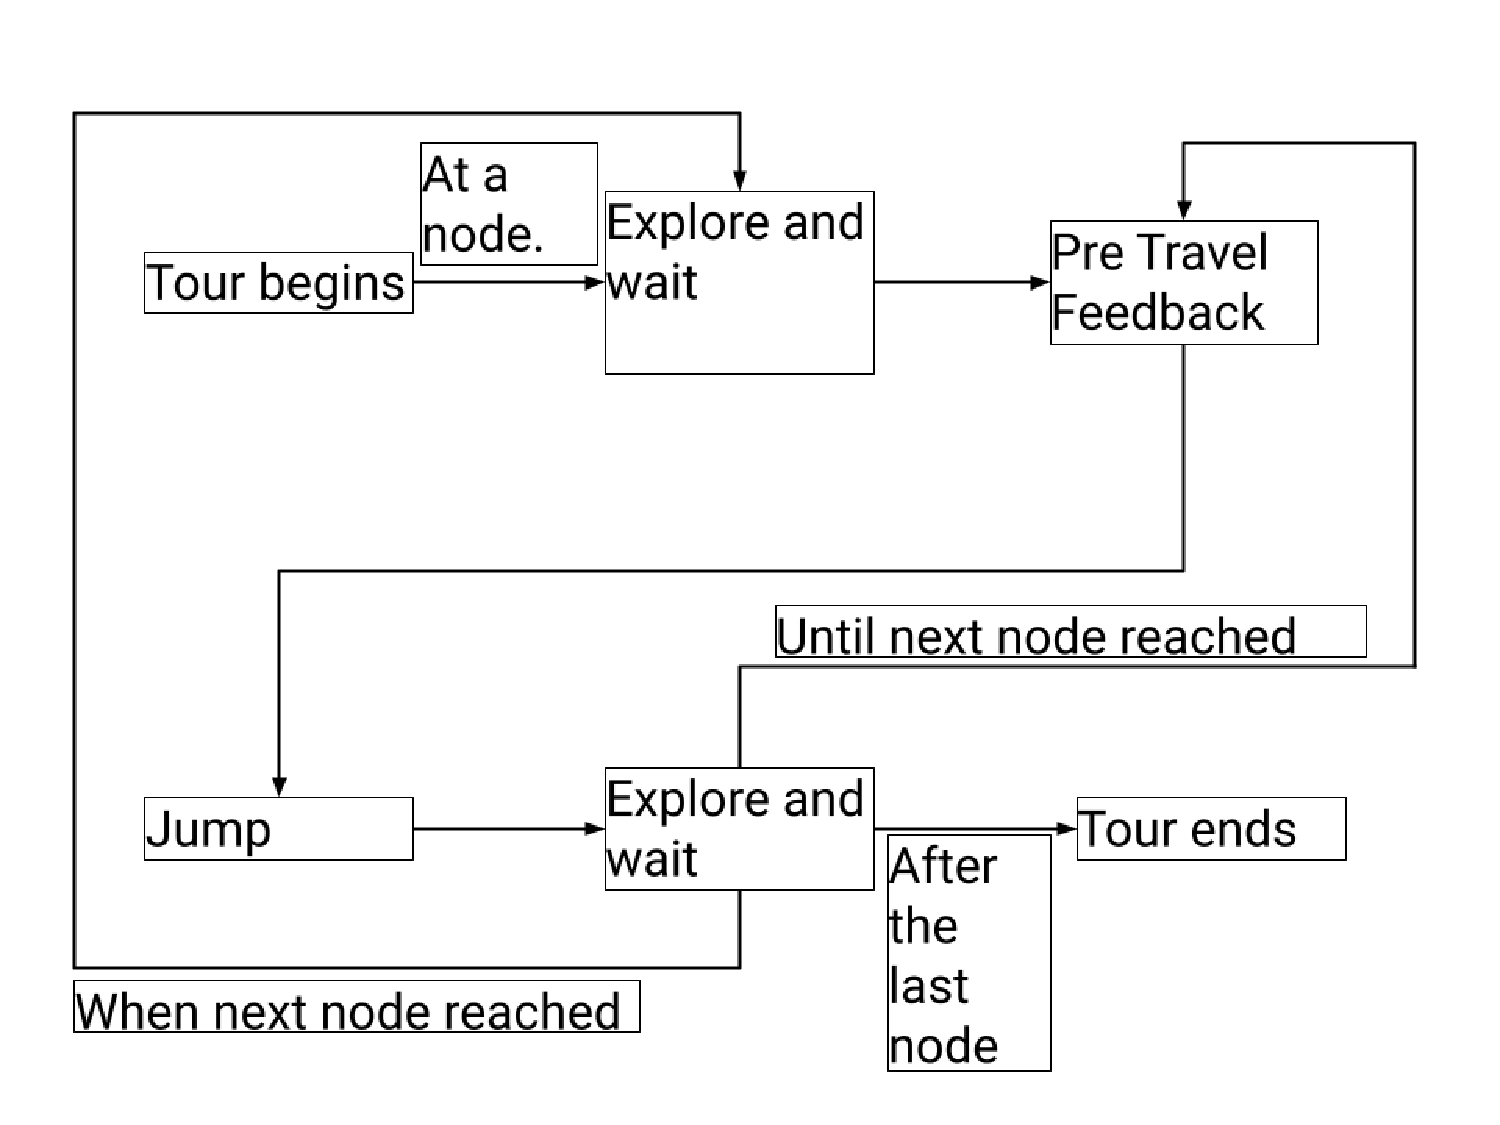
\includegraphics[width=0.75\textwidth]{images/interaction-design-steps.pdf}
	\caption{Steps that would be followed in an exploration of a \acrshort{ve} using the automated guided jumping navigation technique.}
	\label{fig:interaction-design-steps}
\end{figure}

\subsubsection{Travel Feedback}
\label{subsubsection AGJ ID ES: Travel Feedback}
Before a jump takes place, a user needs to know the following information:
\begin{itemize}
	\item The location they will jump to.
	\item Their orientation after the jump.
	\item The time left until the jump takes place.
	\item Whether the guided jumping is paused, allowing them to explore.
\end{itemize}

\subsubsection{Pause to Explore}
\label{subsubsection AGJ ID ES: Pause to Explore}
As the jumping is done automatically, it is important to provide the user with some way to control the technique. This can be done by allowing them to somehow pause the jumping, either implicitly or explicitly so that they can take the time to explore or look around rather than being worried about automatically moving to the next position. Similarly, users would then also have the ability to implicitly or explicitly resume once they are ready to continue. Resuming would reset the countdown to a jump, to avoid sudden jumps after resuming. Looking away from the next node implicitly pauses the guiding and looking back at it resumes it, as looking around is a natural behavior that someone may use to explore an environment. Explicitly pausing or resuming the guiding requires some form of conscious user input, required instead.    

\subsubsection{Choice between Nodes}
\label{subsubsection AGJ ID ES: Choice between Nodes}
In addition to users having the option to pause, users should also have some control over the path they take. This can be provided by adding some nodes that give a choice to the users between multiple possible nodes they can go to. Users get information and travel feedback about each node, and then they can select their preferred node from the given options. 

\section{Environment Setup}
\label{section AGJ: Environment Setup}

Once we came up with a suitable interaction design for the technique, we had to decide how an environment would need to be set up to use this technique. \cref{fig:interaction-design-layout} shows a basic environment in which our guided jumping technique can be used. As mentioned in \cref{subsection AGJ ID: Exploration Steps}, a user has to travel from one node to the next. As nodes are points of interest and can be far apart from each other, to ensure short jumps there are way-points between them. \cref{fig:interaction-design-layout} shows these nodes as and way-points as black and yellow spheres, respectively. As we see in \cref{subsubsection AGJ ID ES: Choice between Nodes}, sometimes there can be more than one node to choose from as the next node. This is indicated in the figure through numbers and arrows.     
\begin{figure}[]
	\centering
	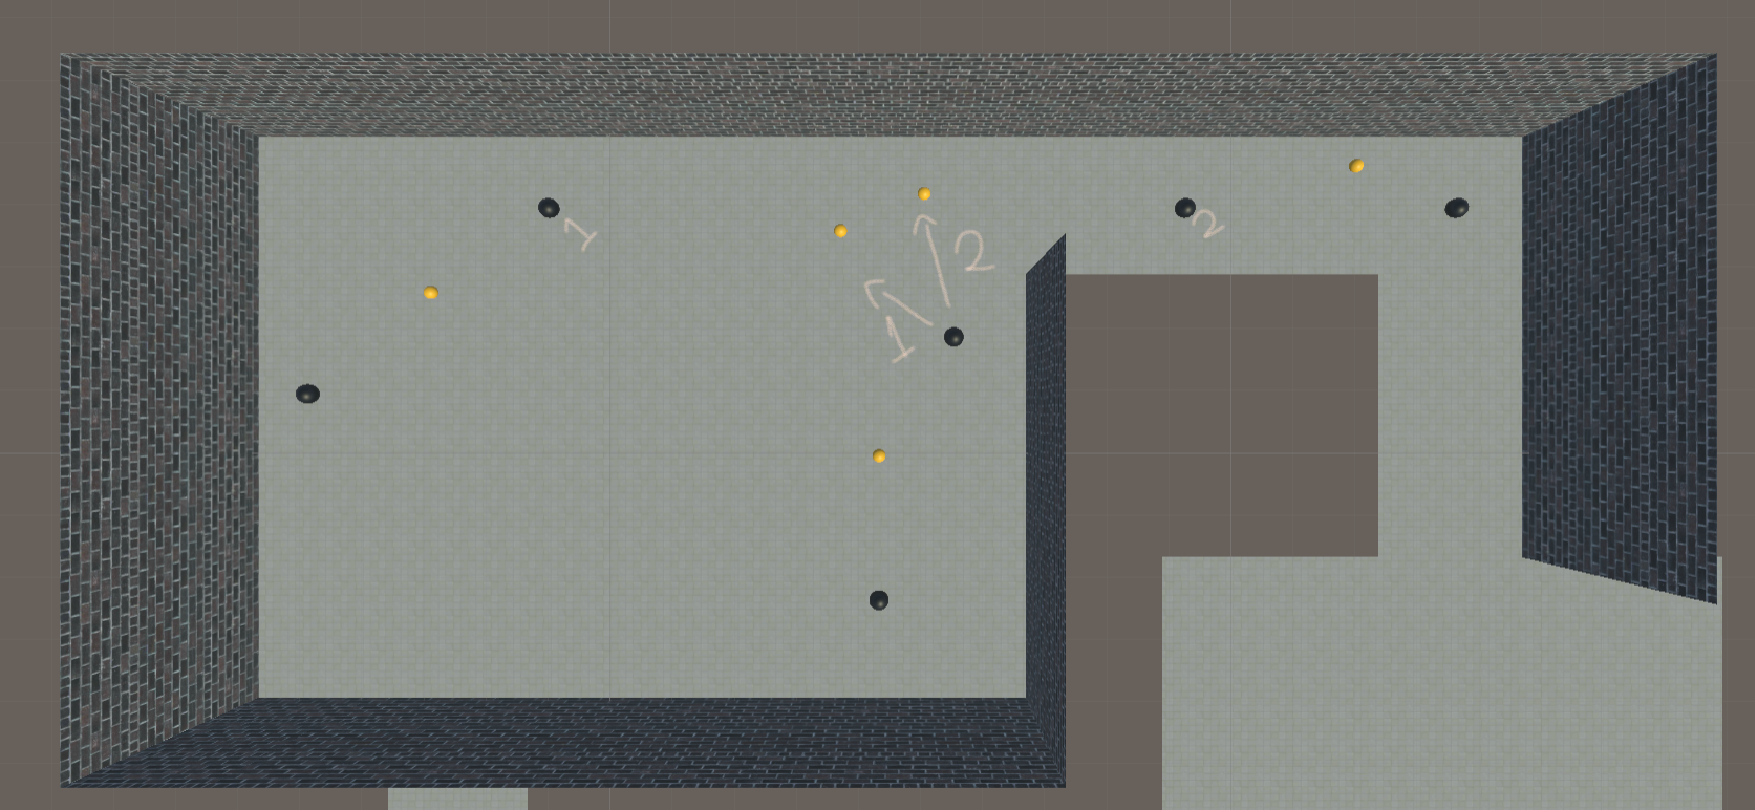
\includegraphics[width=0.5\textwidth]{images/interaction-design-layout.pdf} 
	\caption{This is a potential setup of an environment in which the automated guided jumping navigation would be used. Black spheres = nodes, yellow spheres = way-points, arrows and numbers where there is a choice between nodes}
	\label{fig:interaction-design-layout}
\end{figure}

This environment setup with nodes, way-points and choices is something that would be a part of the environment design by the creator of an experience or tour. The nodes have to be points of interest so should be placed where there is some exhibit or interesting object for users to look at. Nodes should be linked to their next node by giving them index values. Way-points should also be set up between the nodes. Lastly, any nodes where there can be a  choice of next node between more than one node should be set up accordingly with the same index value but different choice number and next node.
 
\section{Automated Jumping}
\label{section AGJ: Automated Jumping}
An environment that is ready with nodes and way-points can use the automated jumping technique. The technique works by moving a user from each way-point or node to the next, while keeping in mind important aspects of teleportation techniques. These are specified by Weissker et al. as: \textit{'target specification, pre-travel information, transitions and post-travel feedback'}~\cite{Weissker2018} and are what make the jumps comprehensible.

\subsection{Comprehensibility of Jumps}
\label{subsection AGJ AJ: Comprehensibility of Jumps}
The target specification in this case is automatic and has been preassigned as the next node or way-point, except for when there is a choice between more than one way-point or node as the next target. Pre-travel information is provided as avatars positioned at the target's location and facing the direction that a user would be oriented towards after a jump. In addition, the time left till the jump will take place is also indicated by a line that gets narrower proportional to the time left. This can be seen in \cref{fig:automated-jumping-feedback}. We decided to go with simple instant transitions for the jumps. There is no specific post-travel feedback, however, after a jump users can already see the pre-travel information for the next jump and are therefore aware that they have completed the current jump. 

\begin{figure}[]
	\centering
	(\centering 1) {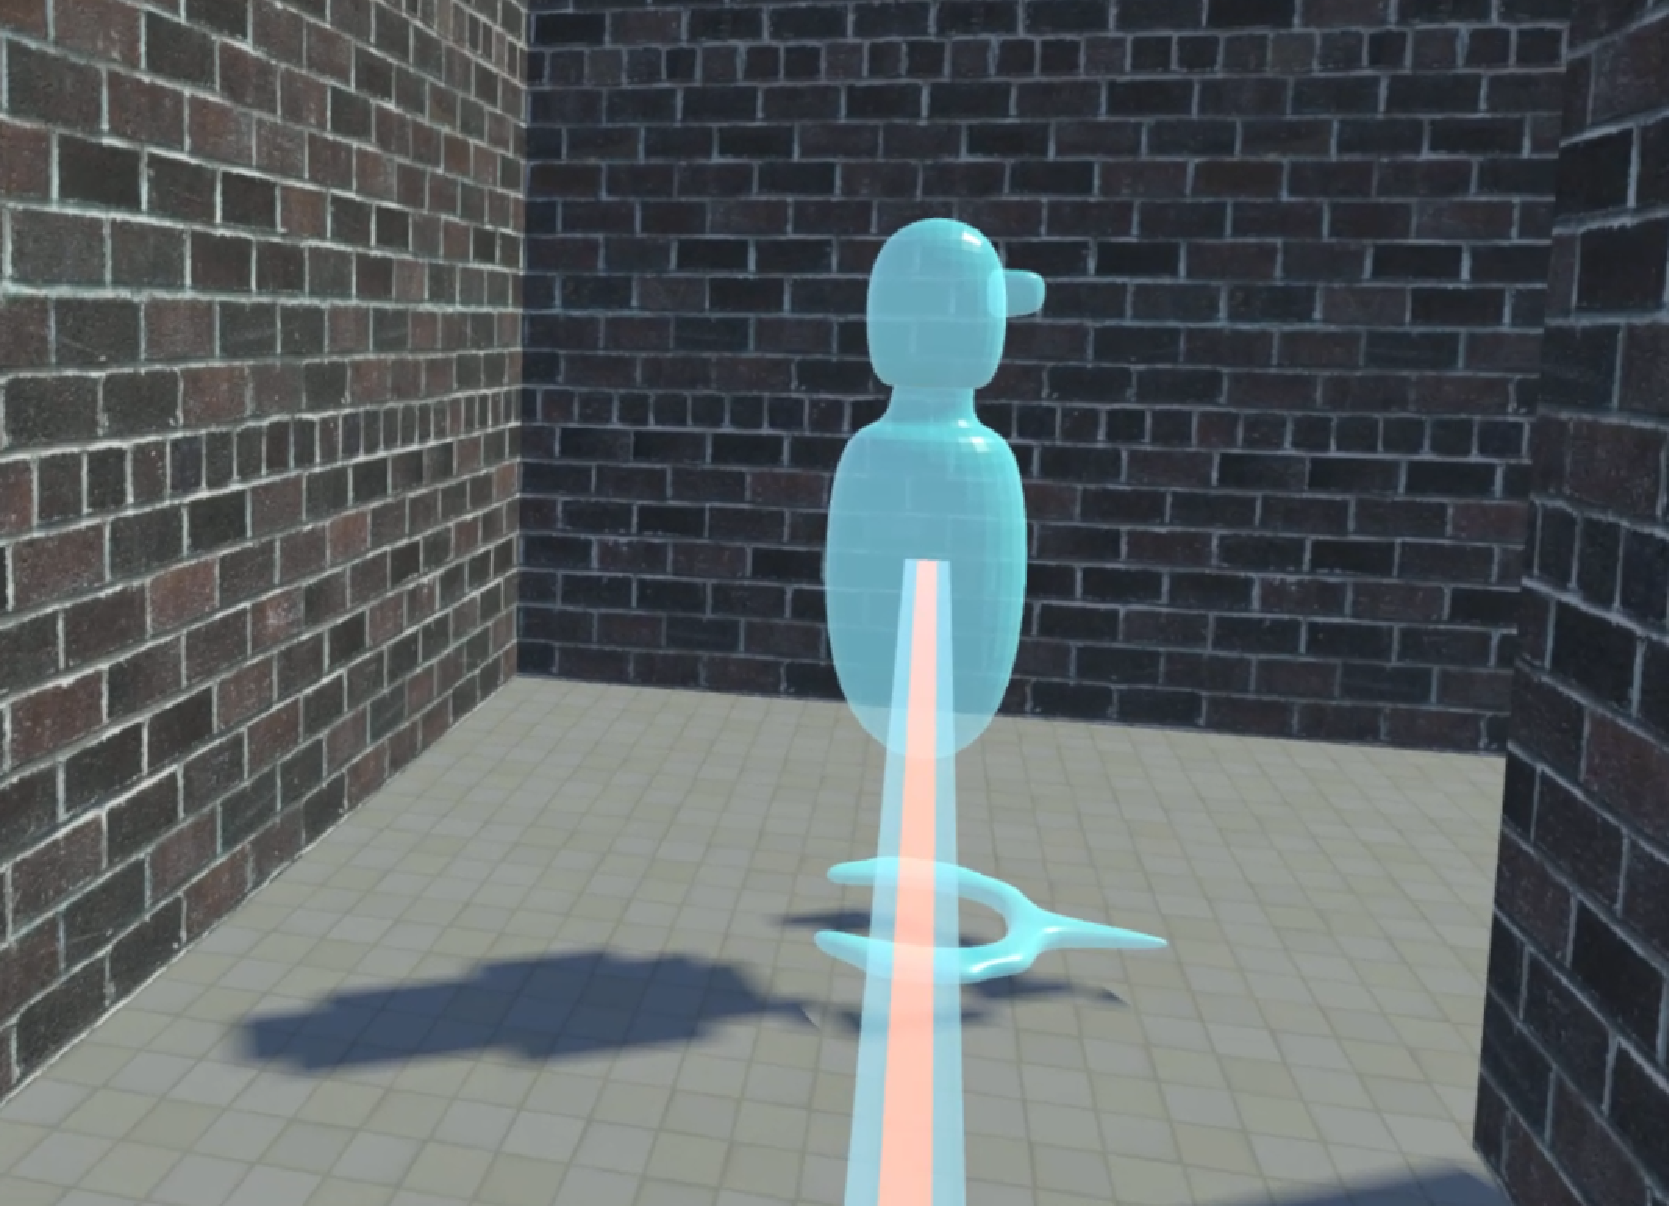
\includegraphics[width=0.25\textwidth]{images/automated-jumping-feedback-1.pdf}}
	(\centering 2) {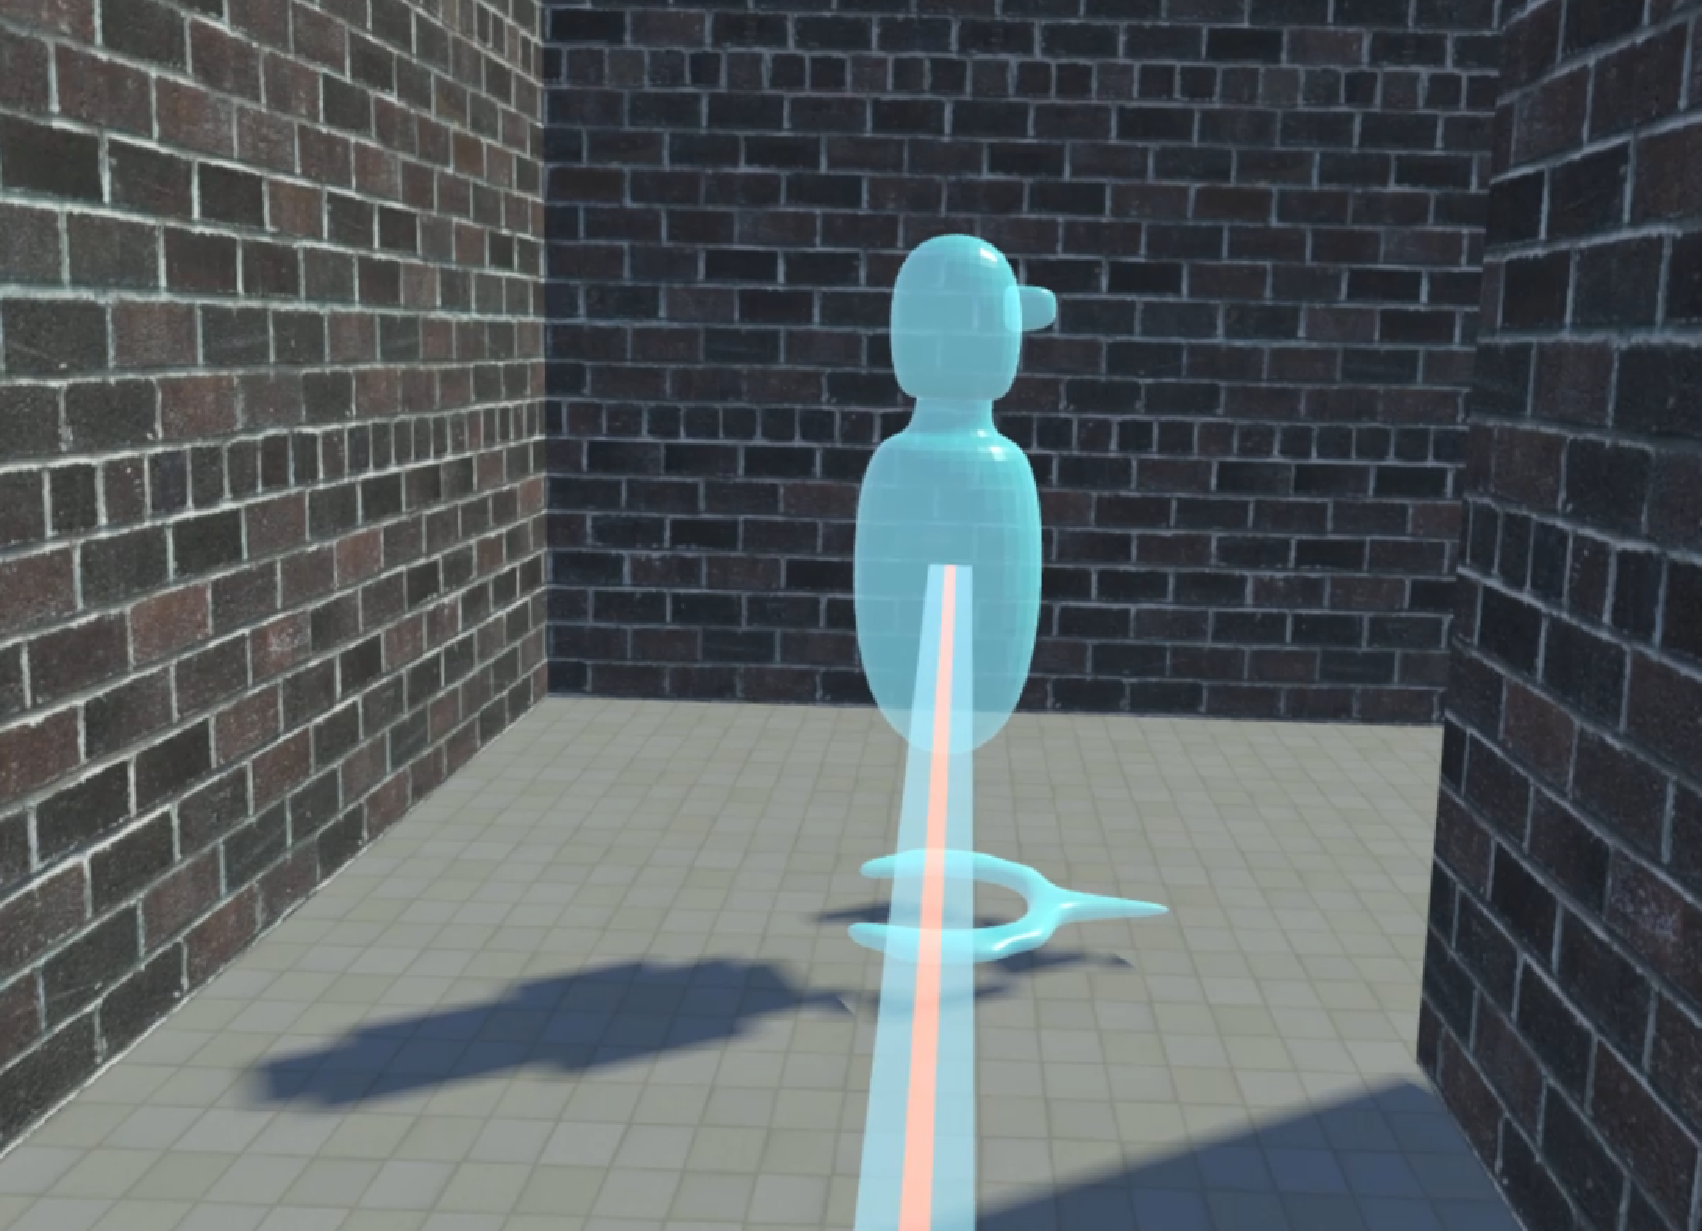
\includegraphics[width=0.25\textwidth]{images/automated-jumping-feedback-2.pdf}} 
	\caption{Avatar at target position facing orientation the user will face after jump. The orange line can be seen to decrease in width between (1) and (2) indicating time left till jump.}
	\label{fig:automated-jumping-feedback}
\end{figure}  

Finally, there has to be feedback when the user has to make a choice or when they pause the automated jumping. This feedback is provided through \acrfull{ui}. To indicate a choice that needs to be made by the user for what path they want to take, there is a combination of arrows and signs pointing to the avatars that indicate the next possible positions to choose from. On selection, a sign that says \textit{'Selected!'} is used to show which option has been selected. In addition, the arrow and sign for the option that is not selected disappear. Once feedback has been given for making a choice, the guiding continues with the node or way-point represented by the selected avatar as the next node or way-point. To indicate that the automatic guiding is paused, a sign that says \textit{'Paused'} becomes visible. \cref{fig:automated-jumping-feedback-ui} shows the different \acrshort{ui}'s for feedback on pausing or making a choice. 

\begin{figure}[]
	\centering
	(\centering 1) {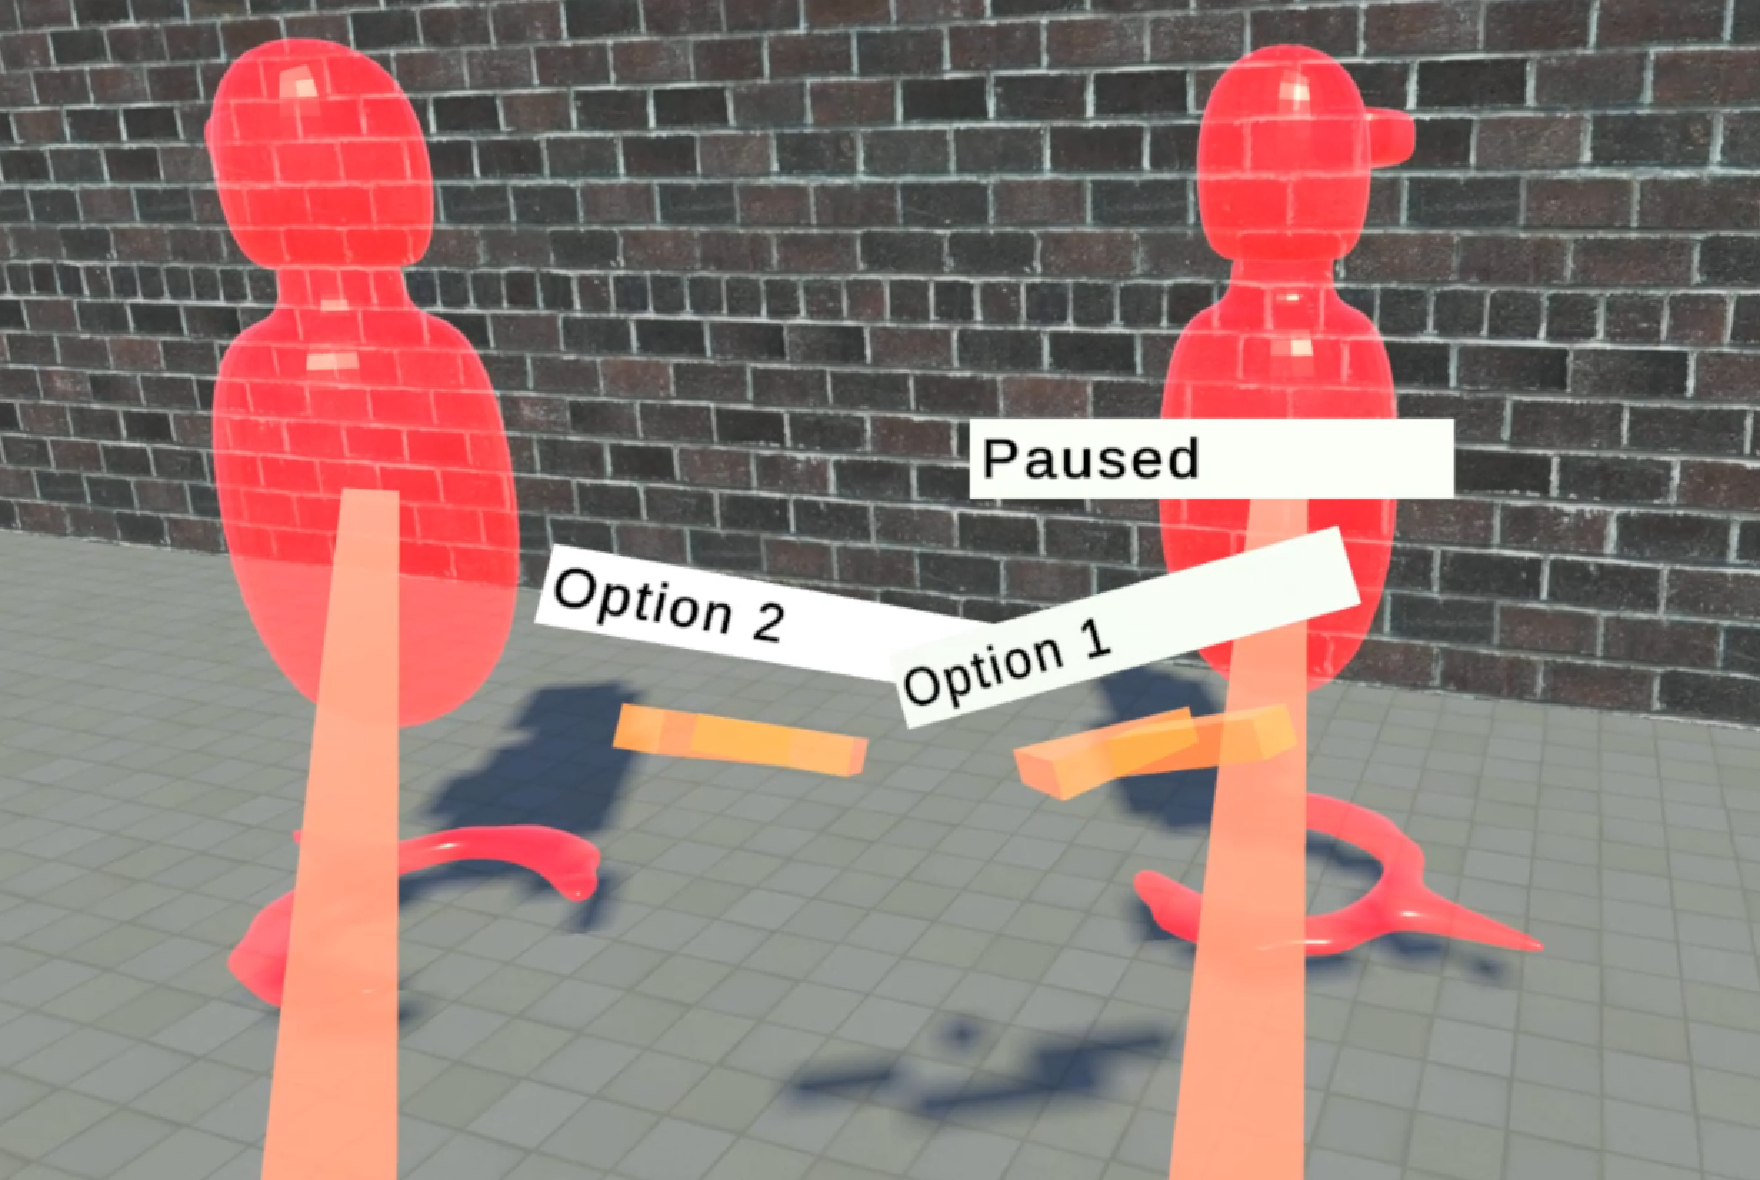
\includegraphics[width=0.25\textwidth]{images/choose.pdf}}
	(\centering 2) {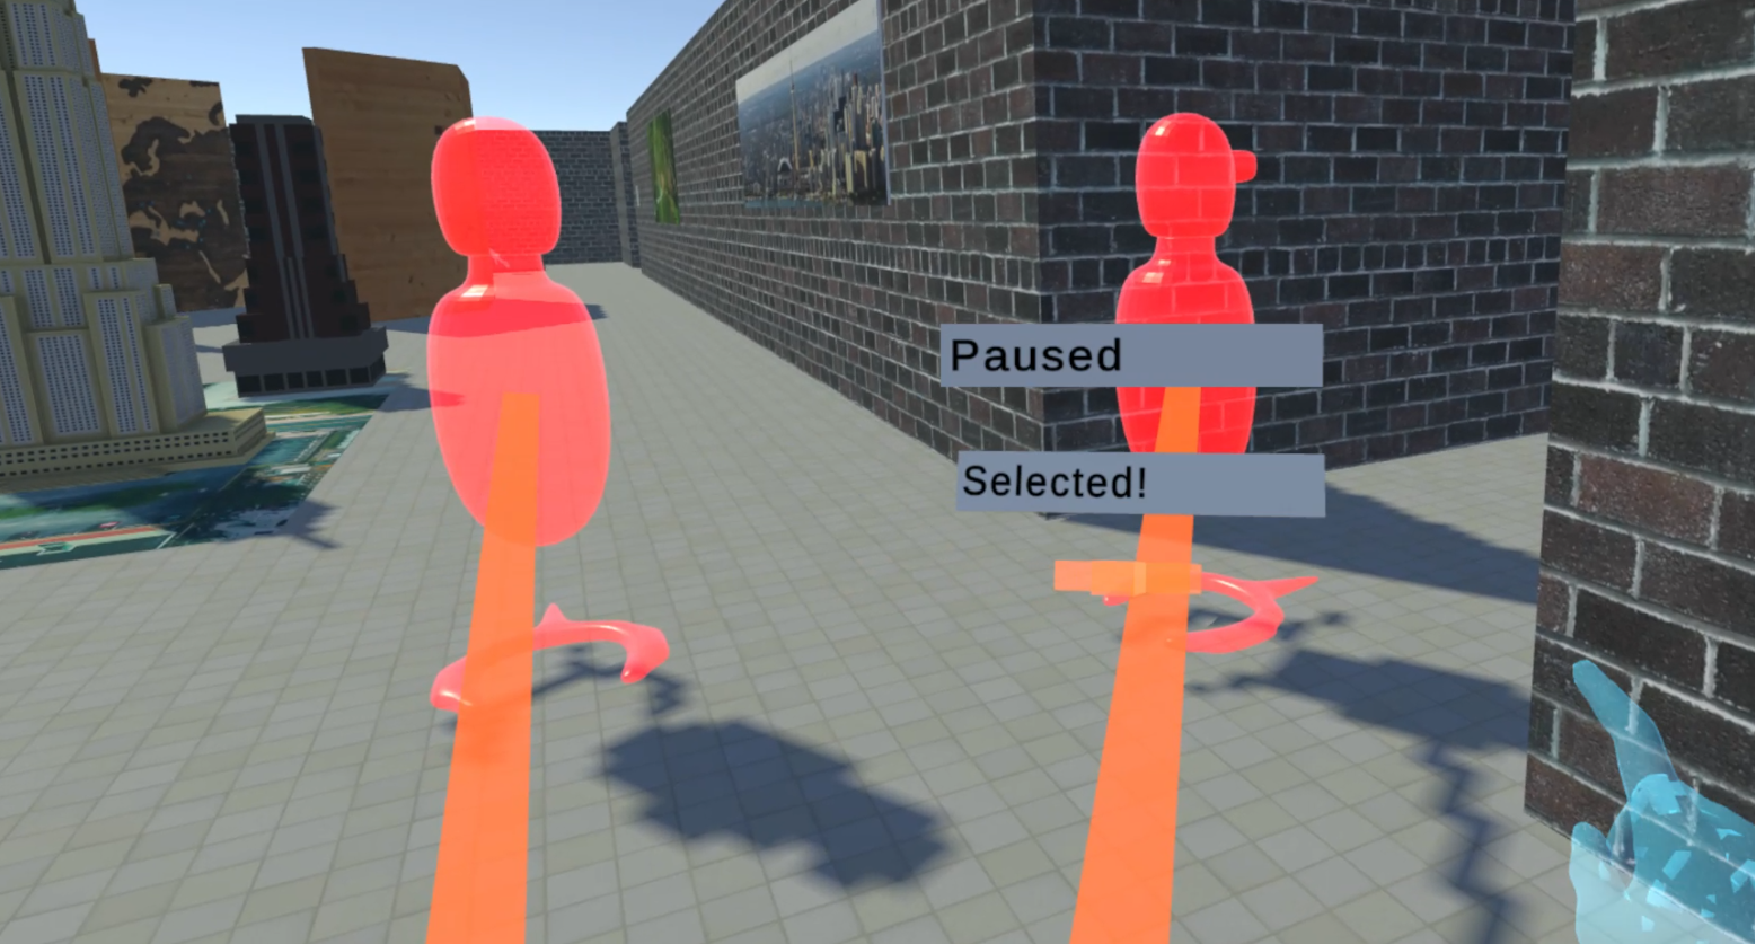
\includegraphics[width=0.25\textwidth]{images/choice-made.pdf}}
	(\centering 3) {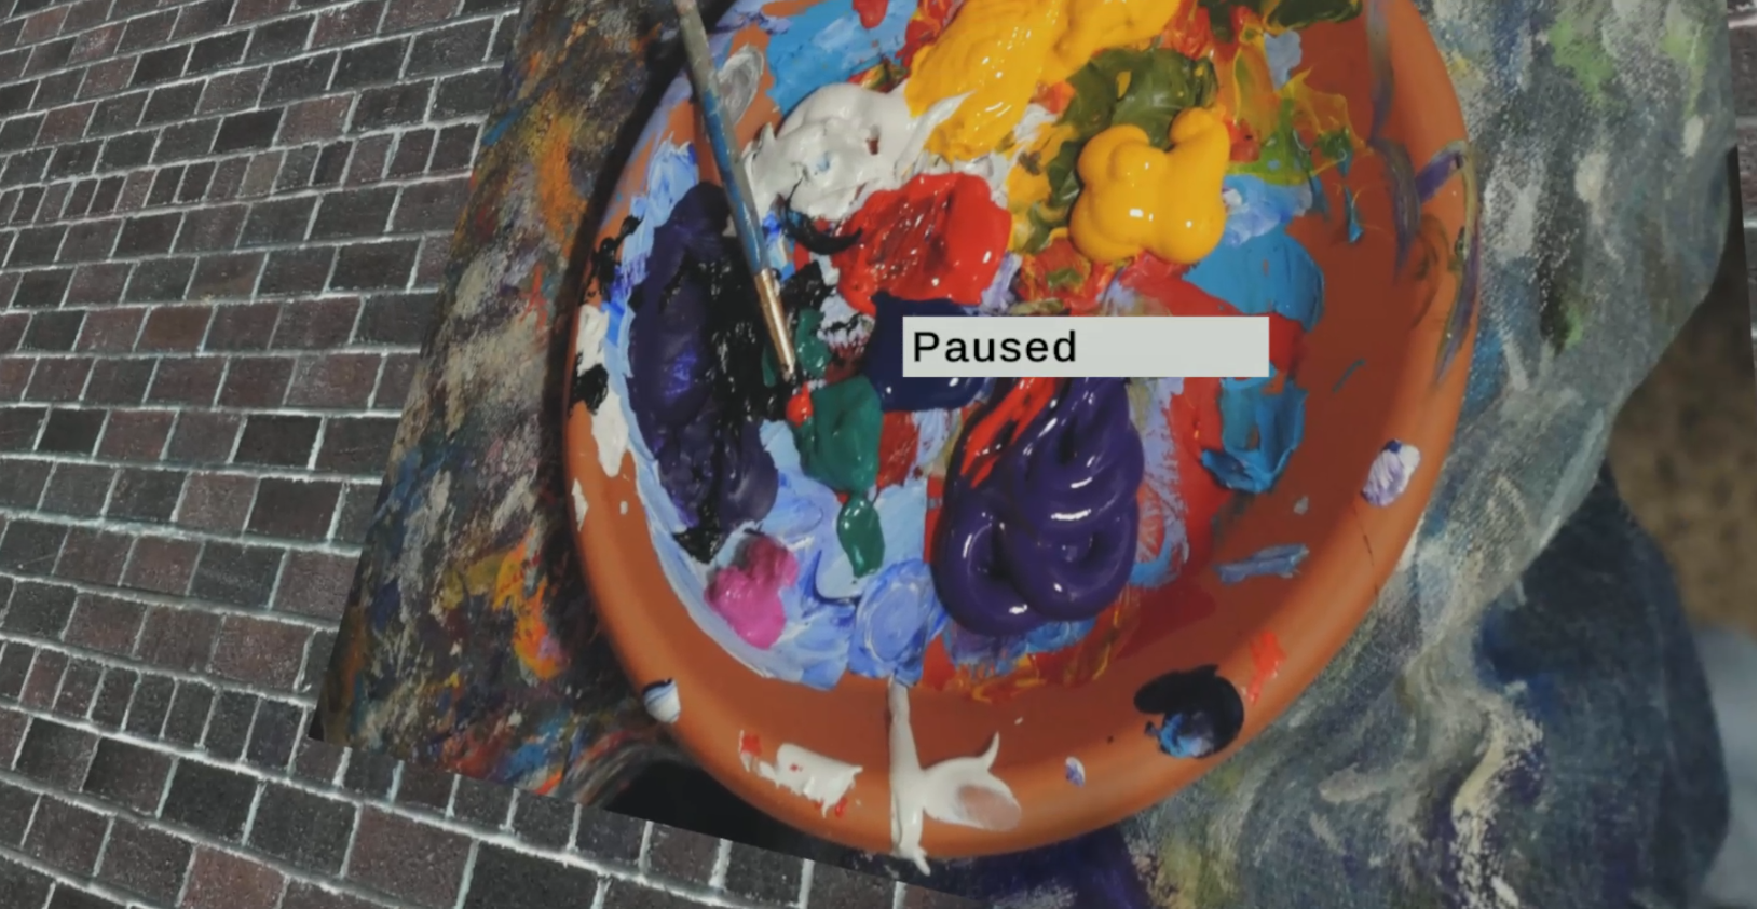
\includegraphics[width=0.25\textwidth]{images/paused.pdf}} 
	\caption{Feedback when making a choice or pausing: (1) Arrows and signs pointing to the different avatars, indicating a choice. (2) The selected avatar is indicated by a sign, while the arrow and sign for the avatar not selected disappear. (3) A sign showing that automated jumping has been paused.}
	\label{fig:automated-jumping-feedback-ui}
\end{figure} 

\subsection{Gesture Control}
\label{subsection AGJ AJ: Gesture Control}
Since we wanted to reduce the learning difficulty for users and also the hardware that would be required to use the technique, we decided on allowing users to use hand gestures with a \acrshort{hmd} that allows for gesture tracking. Users can pause and resume the automated guiding explicitly through hand gestures. They can also use a pointing hand gesture to choose the next node or way-point when there is a choice between more than one. These hand gestures should be natural and represent how a person may do a similar action in a non-virtual environment. \cref{fig:automated-jumping-gestures} shows the hand gestures being used in our \acrshort{ve} using an Oculus Quest 2.
\begin{figure}[]
	\centering
	(\centering 1) {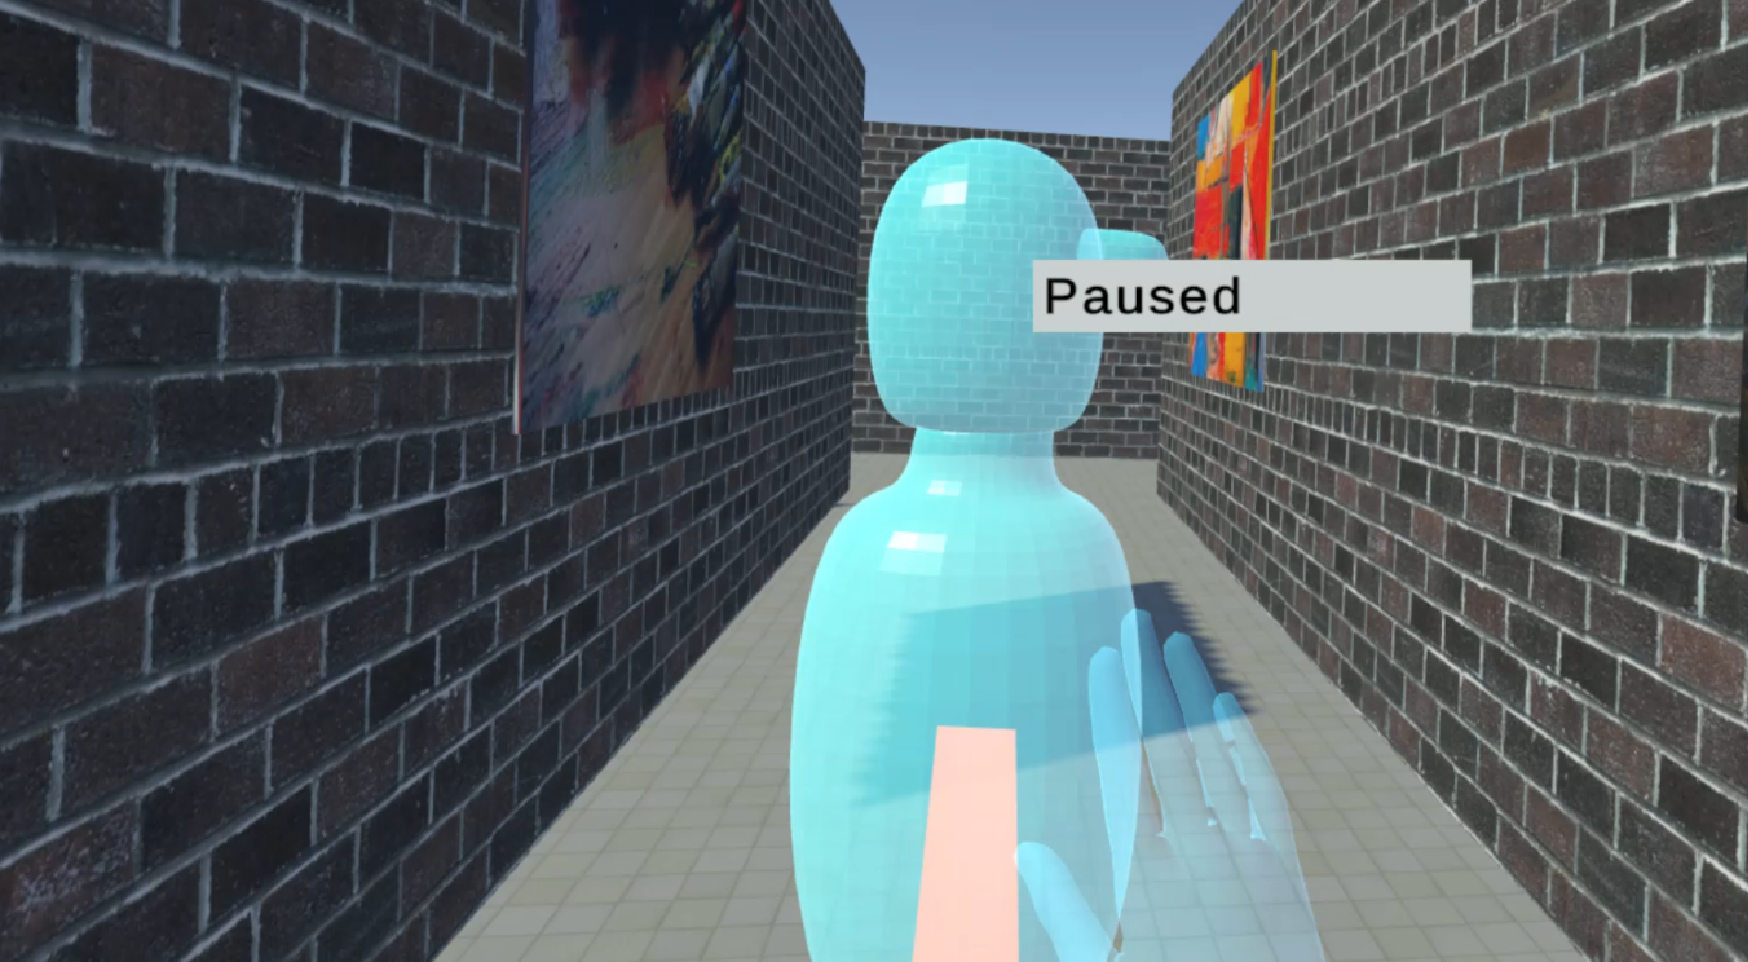
\includegraphics[width=0.25\textwidth]{images/paused-gesture.pdf}}
	(\centering 2) {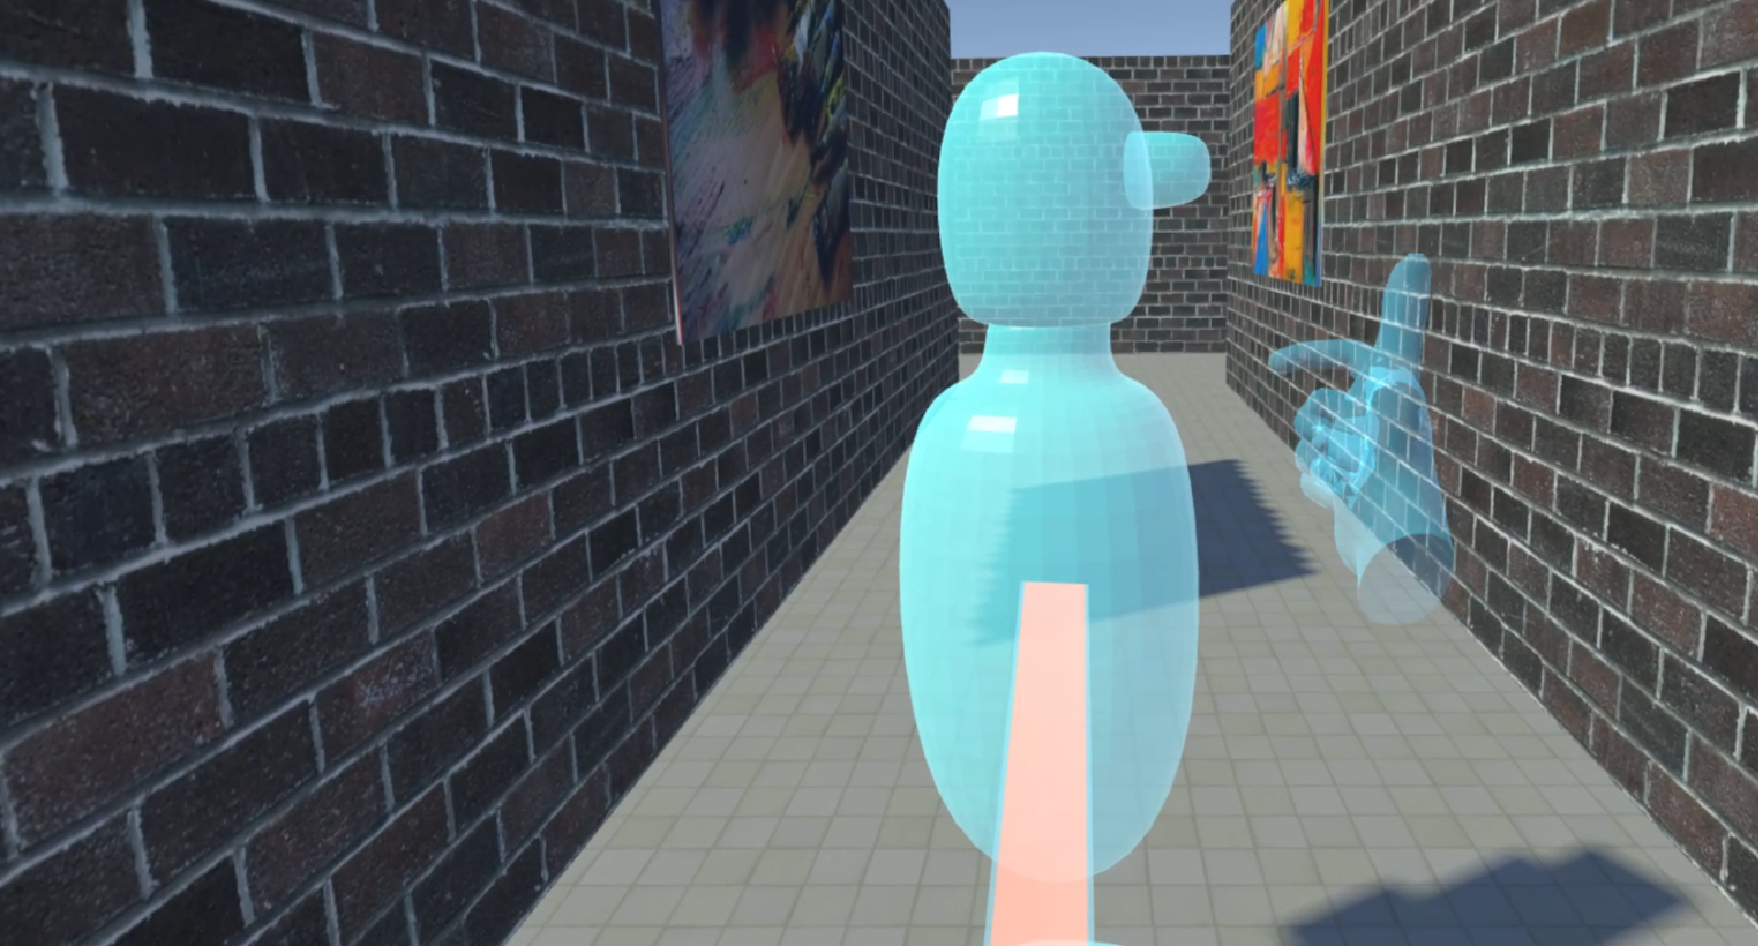
\includegraphics[width=0.25\textwidth]{images/resume-gesture.pdf}}
	(\centering 3) {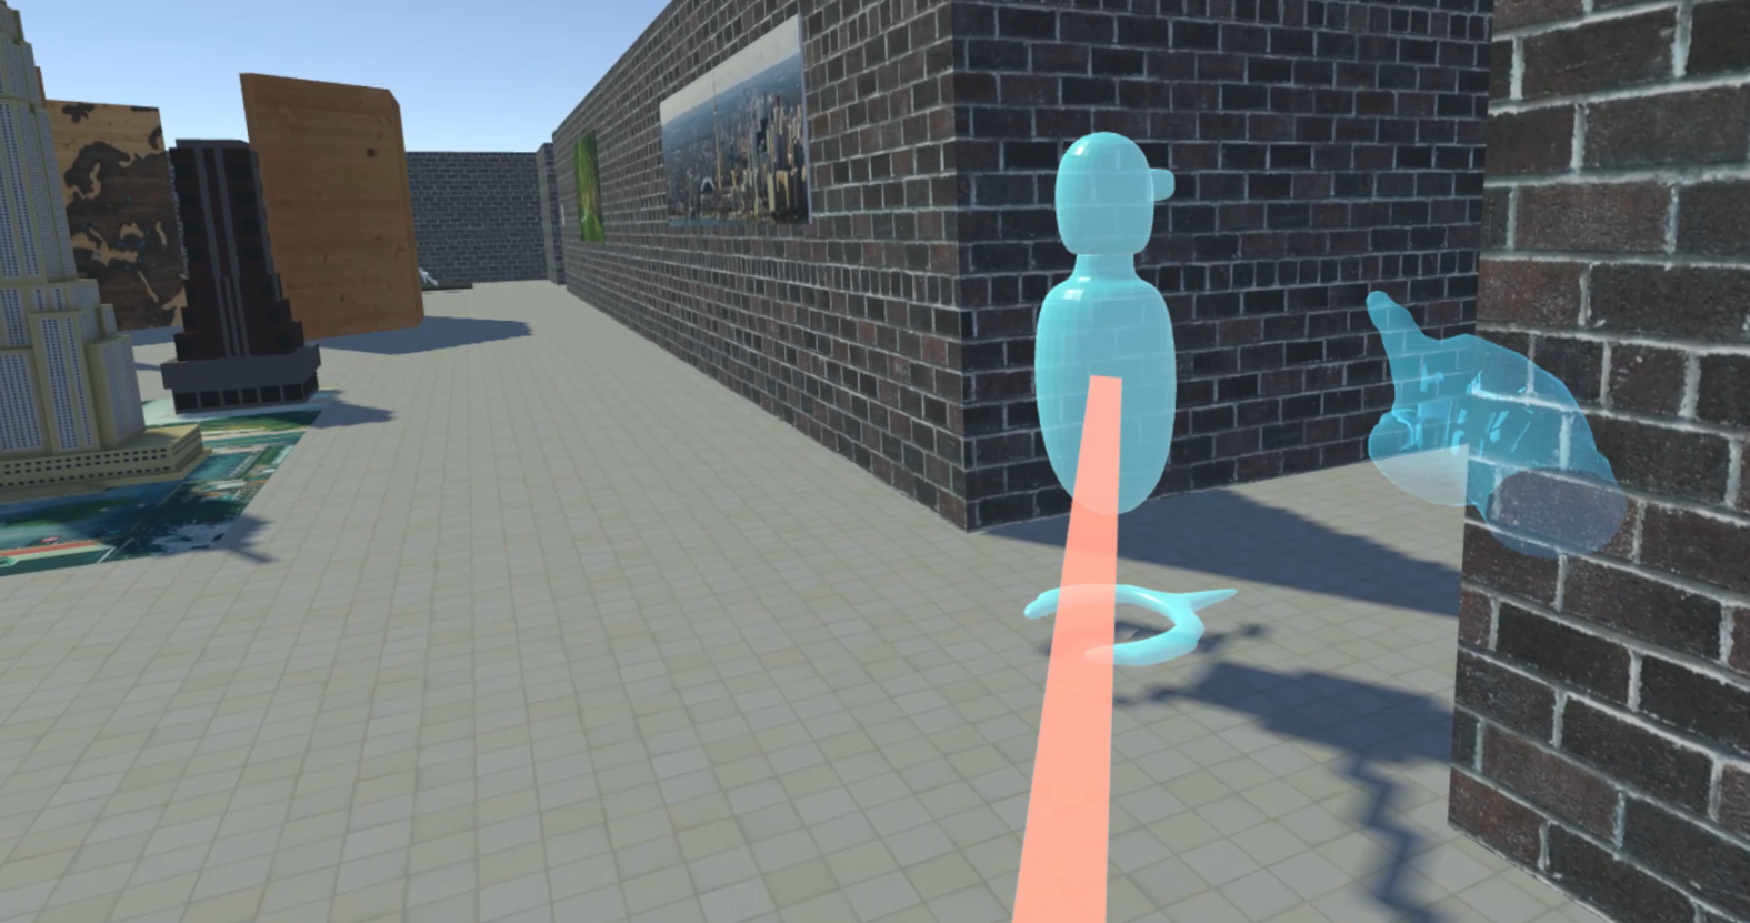
\includegraphics[width=0.25\textwidth]{images/choice-gesture.pdf}} 
	\caption{Gesture control to (1) pause, (2) resume and (3) make a choice.}
	\label{fig:automated-jumping-gestures}
\end{figure} 